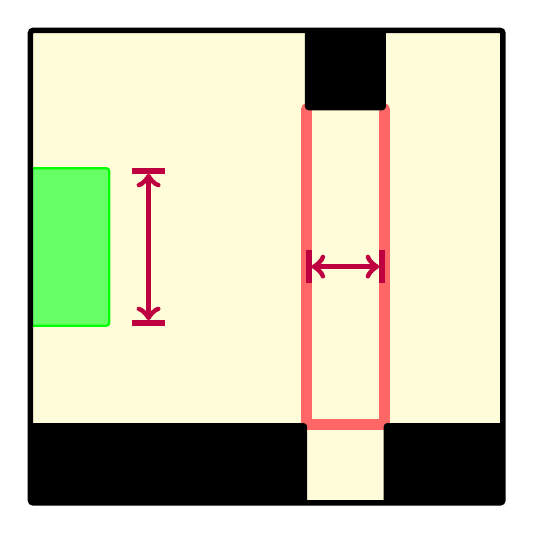
\begin{tikzpicture}[thick,scale=1, every node/.style={scale=1}]

\begin{scope}

\clip (0,0) -- (6,0) -- (6,6) -- (0,6) -- cycle;

\draw [line width=0,fill=yellow!15!white] (0,0) -- (6,0) -- (6,6) -- (0,6) -- cycle;

\draw [red!60!white,line width=4,line cap=round] (3.5,1) -- (3.5,5);
\draw [red!60!white,line width=4,line cap=round] (4.5,5) -- (4.5,1);
\draw [red!60!white,line width=4,line cap=round] (3.5,1) -- (4.5,1);

\draw [fill=black,rounded corners=1] (0,0) -- (0,1) -- (3.5,1) -- (3.5,0) -- cycle;
\draw [fill=black,rounded corners=1] (4.5,0) -- (4.5,1) -- (8,1) -- (8,0) -- cycle;
\draw [fill=black,rounded corners=1] (3.5,5) -- (3.5,6) -- (4.5,6) -- (4.5,5) -- cycle;

\draw [green,fill=green!60!white,rounded corners=1,shift={(1,-0.75)}] (-3,3) -- (-3,5) -- (0,5) -- (0,3) -- cycle;

\draw [arrows=|<->|,purple,line width=2pt,line cap=round,shift={(1,-0.75)}] (0.5,5) -- (0.5,3);
\draw [arrows=|<->|,purple,line width=2pt,line cap=round] (3.5,3) -- (4.5,3);

\end{scope}

\draw [line width=2,rounded corners=1] (0,0) -- (6,0) -- (6,6) -- (0,6) -- cycle;

\end{tikzpicture}